\chapter{Pion photoproduction}\label{sec:PionPhotoproduction}
We now consider the case of pion photoproduction. In the model mentioned in section \ref{sec:model} the nucleon is in a superposition of states with an arbitrary number of pions. However, we constrain the model to the one-pion approximation. This is illustrated in figure \ref{Multicomponent}
\begin{marginfigure}
	\centering
	

% Pattern Info

\tikzset{
	pattern size/.store in=\mcSize, 
	pattern size = 5pt,
	pattern thickness/.store in=\mcThickness, 
	pattern thickness = 0.3pt,
	pattern radius/.store in=\mcRadius, 
	pattern radius = 1pt}
\makeatletter
\pgfutil@ifundefined{pgf@pattern@name@_t53nej2q6}{
	\makeatletter
	\pgfdeclarepatternformonly[\mcRadius,\mcThickness,\mcSize]{_t53nej2q6}
	{\pgfpoint{-0.5*\mcSize}{-0.5*\mcSize}}
	{\pgfpoint{0.5*\mcSize}{0.5*\mcSize}}
	{\pgfpoint{\mcSize}{\mcSize}}
	{
		\pgfsetcolor{\tikz@pattern@color}
		\pgfsetlinewidth{\mcThickness}
		\pgfpathcircle\pgfpointorigin{\mcRadius}
		\pgfusepath{stroke}
}}
\makeatother
\tikzset{every picture/.style={line width=0.75pt}} %set default line width to 0.75pt        

\begin{tikzpicture}[x=0.75pt,y=0.75pt,yscale=-1,xscale=1]
	%uncomment if require: \path (0,389); %set diagram left start at 0, and has height of 389
	
	%Flowchart: Connector [id:dp12351893787926194] 
	\draw  [color={rgb, 255:red, 208; green, 2; blue, 27 }  ,draw opacity=1 ][pattern=_t53nej2q6,pattern size=2.925pt,pattern thickness=0.75pt,pattern radius=0.75pt, pattern color={rgb, 255:red, 208; green, 2; blue, 27}][line width=0.75]  (315.75,205) .. controls (315.75,154.6) and (356.6,113.75) .. (407,113.75) .. controls (457.4,113.75) and (498.25,154.6) .. (498.25,205) .. controls (498.25,255.4) and (457.4,296.25) .. (407,296.25) .. controls (356.6,296.25) and (315.75,255.4) .. (315.75,205) -- cycle ;
	%Flowchart: Connector [id:dp2648272257538774] 
	\draw  [color={rgb, 255:red, 0; green, 0; blue, 0 }  ,draw opacity=1 ][fill={rgb, 255:red, 126; green, 211; blue, 33 }  ,fill opacity=1 ][line width=0.75]  (379,205) .. controls (379,189.54) and (391.54,177) .. (407,177) .. controls (422.46,177) and (435,189.54) .. (435,205) .. controls (435,220.46) and (422.46,233) .. (407,233) .. controls (391.54,233) and (379,220.46) .. (379,205) -- cycle ;
	%Shape: Circle [id:dp5293194247132722] 
	\draw  [fill={rgb, 255:red, 255; green, 255; blue, 255 }  ,fill opacity=1 ] (397,151) .. controls (397,145.48) and (401.48,141) .. (407,141) .. controls (412.52,141) and (417,145.48) .. (417,151) .. controls (417,156.52) and (412.52,161) .. (407,161) .. controls (401.48,161) and (397,156.52) .. (397,151) -- cycle ;
	
	% Text Node
	\draw (400,200) node [anchor=north west][inner sep=0.75pt]  [color={rgb, 255:red, 0; green, 0; blue, 0 }  ,opacity=1 ]  {$N$};
	% Text Node
	\draw (401,147) node [anchor=north west][inner sep=0.75pt]  [color={rgb, 255:red, 0; green, 0; blue, 0 }  ,opacity=1 ]  {$\pi $};
	
	
\end{tikzpicture}
	\caption{Illustration of the dressed nucleon. In the centre (green) is a nucleon, and surrounding it is a cloud of virtual pions (red gradient). }
	\label{Multicomponent}
\end{marginfigure}
There are four pion photoproduction processes on nucleons, and these are given by
\begin{align}
	p \gamma & \rightarrow p \pi^0 \label{photonew1}\\
	p \gamma & \rightarrow n \pi^+ \label{photonew2}\\
	n \gamma & \rightarrow n \pi^0 \label{photonew3}\\
	n \gamma & \rightarrow p \pi^- \label{photonew4}.
\end{align}
Within the framework of this model, we would expect these processes by applying the equation \eqref{isocoeff} to the isospin state of the given nucleon, i.e
\begin{equation} \label{isovectorex}
	(\vec{\tau}\cdot\vec{\pi}) p = p\pi^0 + \sqrt{2}n\pi^+,
\end{equation}
and similarly for the isospin state of the neutron. As mentioned in section \ref{sec:DressingofProton} the pion is trapped behind a potential barrier of height $140$ MeV and cannot leave unless an incoming photon of sufficient energy hits the pion-nucleon system and photodisintegrates the virtual pion and creates a physical pion in the process. This means pion photoproduction comes naturally as a photodisintegration process. Consider some initial bound state represented by the following two-component wave function
\begin{equation} \label{phii}
	\ket{\Phi_i} = \mqty[\phi_p \\ \phi_{N\pi}],
\end{equation}
where $\phi$ represents a bound state. The final state consists of the same superposition but in an unbound system represented by $\psi$, i.e.
\begin{equation} \label{psif}
	\ket{\Psi_f} = \mqty[\psi_p \\ \psi_{N\pi}].
\end{equation}
The two-component wave function photodisintegration is similar to the photodisintegration process of the deuteron\footnote{This is covered in appendix \ref{app:deuteron}}. We can apply a similar approach and get an expression for the total cross section as a function of energy and the strength parameter $S$, and the range parameter $b$. The general idea is to fit the parameters to experimental data such that we get a set of parameters within which the model can describe the total cross-section near the threshold. We constrain the model to only apply near the threshold since we expect more pions are needed to describe the total cross section at higher energies adequately.
The advantages of this model are twofold: the reduced number of parameters allows us to fit the model to experimental data efficiently, and the model's generality will enable us to apply these parameters to a different process accounting only for the difference in mass and isospin coefficient. Also, in the case of the pion photoproduction process \eqref{photonew1} is very well investigated while \eqref{photonew2} and \eqref{photonew1} have limited data and \eqref{photonew3} have none near the threshold. Our first approach is to apply a dipole approximation since we are considering the photoproduction processes near the threshold. 
\section{Dipole Approximation}\label{sec:dipoleapprox}
We want to calculate the total cross-section of pion photoproduction off nucleons. In this section, we focus on the process involving charged pions off protons given by equation \eqref{photonew2}. The general idea is to use Fermi's golden rule, and this involves a matrix element expressed in terms of equation \eqref{phii} and equation \eqref{psif}
\begin{equation}\label{dipoleoperator}
	\mel{\Psi_f}{\vec{d}}{\Phi_i},
\end{equation}
where a dipole operator $\vec{d}$. Equation \eqref{dipoleoperator} just means we use the dipole operator on some bound initial state and the final state consists of an unbound system. We start from the general expression of the multi-component wave function and impose a normalisation to both the initial and final state. Starting from \eqref{phii}
\begin{align}\label{finalphi}
	\Phi = \mathcal{N} \mqty[p\uparrow \\ (\vec{\tau}\cdot \vec{\pi})(\vec{\sigma}\cdot \vec{r})p\uparrow \phi(r)],
\end{align}
where $\uparrow$ represents the spin state, $\phi(r)$ is the wave function from figure \ref{fig:integralplot} and $\mathcal{N}$ is the normalisation constant. This leads to
\begin{align}
	\braket{\Phi}{\Phi} &= \abs{\mathcal{N}}^2 \big( \braket{\phi_p}{\phi_p}+ \braket{\phi_{N\pi}}{\phi_{N\pi}} \big) \\
	&= \abs{\mathcal{N}}^2 \big( V+3V\int \text{d}^3r \, r^2 \phi(r)^2 \big)\label{int} \\
	&\stackrel{!}{=} 1.
\end{align} 
This leads to the following normalisation constant
\begin{equation}
	\mathcal{N} = \frac{1}{\sqrt{V}}\frac{1}{\sqrt{1+\epsilon}},
\end{equation}
where $V$ is the volume and $\epsilon$ is the integral in \eqref{int}--numerically, this is close to unity. This expression is the properly normalised initial state. 
\begin{marginfigure}
	\centering
	

\tikzset{every picture/.style={line width=0.75pt}} %set default line width to 0.75pt        

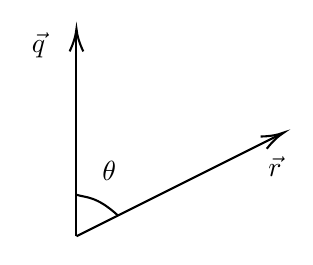
\begin{tikzpicture}[x=0.75pt,y=0.75pt,yscale=-1,xscale=1]
%uncomment if require: \path (0,300); %set diagram left start at 0, and has height of 300

%Straight Lines [id:da4402999370947803] 
\draw    (250,150) -- (250,52) ;
\draw [shift={(250,50)}, rotate = 90] [color={rgb, 255:red, 0; green, 0; blue, 0 }  ][line width=0.75]    (10.93,-3.29) .. controls (6.95,-1.4) and (3.31,-0.3) .. (0,0) .. controls (3.31,0.3) and (6.95,1.4) .. (10.93,3.29)   ;
%Straight Lines [id:da0037929251539179365] 
\draw    (250,150) -- (348.21,100.89) ;
\draw [shift={(350,100)}, rotate = 153.43] [color={rgb, 255:red, 0; green, 0; blue, 0 }  ][line width=0.75]    (10.93,-3.29) .. controls (6.95,-1.4) and (3.31,-0.3) .. (0,0) .. controls (3.31,0.3) and (6.95,1.4) .. (10.93,3.29)   ;
%Curve Lines [id:da06140636400336408] 
\draw    (250,130) .. controls (254.53,131.45) and (259.53,130.45) .. (270,140) ;

% Text Node
\draw (227,50.4) node [anchor=north west][inner sep=0.75pt]    {$\vec{q}$};
% Text Node
\draw (341,110.4) node [anchor=north west][inner sep=0.75pt]    {$\vec{r}$};
% Text Node
\draw (261,112.4) node [anchor=north west][inner sep=0.75pt]    {$\theta $};


\end{tikzpicture}
	\caption{Illustration of the angle between the two vectors $\vec{q}$ and $\vec{r}$ in equation (\ref{expansion})}
	\label{normsphere}
\end{marginfigure}
The final state consists of the unbound system represented by $\psi$. We know the final state consists of a plane wave with wave number $\vec{q}$ propagating along the $z$-axis. The wave number \vec{q} is written in terms of the pion-nucleon momentum and the magnitude of this is given by
\begin{equation}\label{key}
	\frac{\hbar^2 q^2}{2\mu_{N\pi}}=\hbar \omega-m_\pi c^2,
\end{equation}
which is also illustrated in figure \ref{fig:qenergy}. The plane wave can be represented by 
\begin{equation} \label{key}
	\text{e}^{iqz} = \text{e}^{i \vec{q}\cdot \vec{r}},
\end{equation}
where $\theta$ is the angle between $\vec{q}$ and $\vec{r}$ illustrated on \ref{normsphere}. Using orthogonality and the addition theorem for the spherical harmonics, we can decompose the plane wave into a Bessel function and spherical harmonics\footnote{See equation \eqref{sphericalbesseldecomp}}. This yields
\begin{align}\label{planewaveexpansion}
	\frac{1}{\sqrt{V}} \text{e}^{-i\vec{q}\cdot\vec{r}} &= \frac{1}{\sqrt{V}} \sum_{\ell,m} 4\pi i^\ell Y_\ell^{*m}(\vec{q})Y_\ell^m(\vec{r})j_\ell(qr) \\
	&= \frac{1}{\sqrt{V}} \sum_\ell 4\pi i^\ell j_\ell(qr) \bigg( \frac{2\ell+1}{4\pi}\bigg)P_\ell(\cos\theta),
\end{align}
and $P_\ell$ is the Legendre polynomial of degree $\ell$. Since we are considering the energies close to the threshold, we expect mainly the $S$-wave to contribute and ignore higher orders\footnote{Threshold behaviour when $\lambda\simeq1/q\gg R$ where $R$ is the range higher orders of $\ell$ are generally not important \cite{Sakurai}.}. We should empathise that this is an approximation, and a priori, we do not know to what degree this holds. In terms of the expansion \eqref{planewaveexpansion} this greatly simplified the expression
\begin{equation} \label{expansion}
	\frac{1}{\sqrt{V}}\text{e}^{i\vec{q}\cdot \vec{r}} \stackrel{\ell=0}{=} \frac{1}{\sqrt{V}}j_0(qr).
\end{equation}
As equation \eqref{expansion} shows, we are left with a spherical Bessel function in the final state where the volume is kept to stress that the total cross section must be independent of the volume. To calculate the matrix element we return to equation \eqref{quantized} and consider the electric field given by
\begin{equation}\label{EF}
	\vec{\mathcal{E}} = -\frac{1}{c} \frac{\partial \vec{A}}{\partial t}.
\end{equation}
The interaction operator in the dipole approximation is given by
\begin{equation}\label{Dip}
	H_\text{dipole} = -\vec{\mathcal{E}}(\vec{r}=0)\cdot \vec{d},
\end{equation}
where $\vec{d}$ is the dipole moment of the pion-nucleon system given by 
\begin{equation}\label{dipolemoment}
	\vec{d}=e\frac{\mu_{N\pi}}{m_\pi}\vec{r}.
\end{equation}
\begin{marginfigure}
	\centering
	

\tikzset{every picture/.style={line width=0.75pt}} %set default line width to 0.75pt        

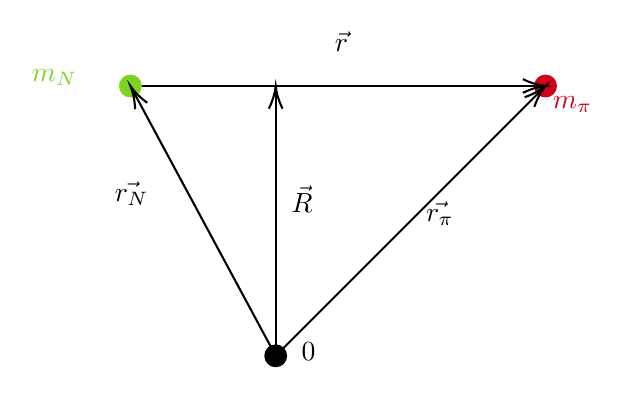
\begin{tikzpicture}[x=0.75pt,y=0.75pt,yscale=-1,xscale=1]
	%uncomment if require: \path (0,300); %set diagram left start at 0, and has height of 300
	
	%Flowchart: Connector [id:dp9827455772611288] 
	\draw  [color={rgb, 255:red, 208; green, 2; blue, 27 }  ,draw opacity=1 ][fill={rgb, 255:red, 208; green, 2; blue, 27 }  ,fill opacity=1 ] (315,90) .. controls (315,87.24) and (317.24,85) .. (320,85) .. controls (322.76,85) and (325,87.24) .. (325,90) .. controls (325,92.76) and (322.76,95) .. (320,95) .. controls (317.24,95) and (315,92.76) .. (315,90) -- cycle ;
	%Straight Lines [id:da5093684133345362] 
	\draw    (125,90) -- (318,90) ;
	\draw [shift={(320,90)}, rotate = 180] [color={rgb, 255:red, 0; green, 0; blue, 0 }  ][line width=0.75]    (10.93,-3.29) .. controls (6.95,-1.4) and (3.31,-0.3) .. (0,0) .. controls (3.31,0.3) and (6.95,1.4) .. (10.93,3.29)   ;
	%Straight Lines [id:da04984112064582158] 
	\draw    (190,220) -- (190,92) ;
	\draw [shift={(190,90)}, rotate = 90] [color={rgb, 255:red, 0; green, 0; blue, 0 }  ][line width=0.75]    (10.93,-3.29) .. controls (6.95,-1.4) and (3.31,-0.3) .. (0,0) .. controls (3.31,0.3) and (6.95,1.4) .. (10.93,3.29)   ;
	%Straight Lines [id:da13661676787341415] 
	\draw    (190,220) -- (318.59,91.41) ;
	\draw [shift={(320,90)}, rotate = 135] [color={rgb, 255:red, 0; green, 0; blue, 0 }  ][line width=0.75]    (10.93,-3.29) .. controls (6.95,-1.4) and (3.31,-0.3) .. (0,0) .. controls (3.31,0.3) and (6.95,1.4) .. (10.93,3.29)   ;
	%Flowchart: Connector [id:dp37210275318157304] 
	\draw  [color={rgb, 255:red, 126; green, 211; blue, 33 }  ,draw opacity=1 ][fill={rgb, 255:red, 126; green, 211; blue, 33 }  ,fill opacity=1 ] (115,90) .. controls (115,87.24) and (117.24,85) .. (120,85) .. controls (122.76,85) and (125,87.24) .. (125,90) .. controls (125,92.76) and (122.76,95) .. (120,95) .. controls (117.24,95) and (115,92.76) .. (115,90) -- cycle ;
	%Straight Lines [id:da8769015497622031] 
	\draw    (190,220) -- (120.95,91.76) ;
	\draw [shift={(120,90)}, rotate = 61.7] [color={rgb, 255:red, 0; green, 0; blue, 0 }  ][line width=0.75]    (10.93,-3.29) .. controls (6.95,-1.4) and (3.31,-0.3) .. (0,0) .. controls (3.31,0.3) and (6.95,1.4) .. (10.93,3.29)   ;
	%Flowchart: Connector [id:dp5562170943538245] 
	\draw  [color={rgb, 255:red, 0; green, 0; blue, 0 }  ,draw opacity=1 ][fill={rgb, 255:red, 0; green, 0; blue, 0 }  ,fill opacity=1 ] (185,220) .. controls (185,217.24) and (187.24,215) .. (190,215) .. controls (192.76,215) and (195,217.24) .. (195,220) .. controls (195,222.76) and (192.76,225) .. (190,225) .. controls (187.24,225) and (185,222.76) .. (185,220) -- cycle ;
	
	% Text Node
	\draw (71,80.4) node [anchor=north west][inner sep=0.75pt]  [color={rgb, 255:red, 126; green, 211; blue, 33 }  ,opacity=1 ]  {$m_{N}$};
	% Text Node
	\draw (322,93.4) node [anchor=north west][inner sep=0.75pt]  [color={rgb, 255:red, 208; green, 2; blue, 27 }  ,opacity=1 ]  {$m_{\pi }$};
	% Text Node
	\draw (196,136.4) node [anchor=north west][inner sep=0.75pt]    {$\vec{R}$};
	% Text Node
	\draw (261,144.4) node [anchor=north west][inner sep=0.75pt]    {$\vec{r_{\pi }}$};
	% Text Node
	\draw (111,134.4) node [anchor=north west][inner sep=0.75pt]    {$\vec{r_{N}}$};
	% Text Node
	\draw (217,62.4) node [anchor=north west][inner sep=0.75pt]    {$\vec{r}$};
	% Text Node
	\draw (201,212.4) node [anchor=north west][inner sep=0.75pt]    {$0$};
	
	
\end{tikzpicture}
	\caption{Relative coordinates of the pion-nucleon system.}
	\label{JacobiIllustration1}
\end{marginfigure}
The general setup for the system is shown in figure \ref{JacobiIllustration1} where the nucleon in this case is a proton. Considering a general pion photoproduction process on the form
\begin{equation}\label{General}
	N+\gamma \rightarrow N+\pi
\end{equation}
allows us to calculate the electromagnetic part of the matrix element. The initial state consists of the dressed nucleon and a photon $a_{\vec{k},\lambda}^\dagger \ket{0}$, where $\ket{0}$ is the electromagnetic vacuum state. The final state consists of a nucleon, a pion and the electromagnetic vacuum. This means the transition in the dipole approximation is given by 
\begin{equation}\label{Dip2}
	\mel{0}{\vec{\mathcal{E}}a_{\vec{k},\lambda}^\dagger}{0} = \sqrt{\frac{2\pi\hbar}{\omega_k V}}i\omega_k \vec{e}_{\vec{k},\lambda}\text{e}^{-i\omega_k t},
\end{equation}
which combined with Fermi's golden rule
\begin{equation}\label{FermiGoldenRule}
	\text{d}\omega = \frac{2\pi}{\hbar}\abs{\mathcal{M}}^2 \text{d}\rho,
\end{equation}
describes the probability per unit of time of making a transition. Equation \eqref{Dip2} is the most general expression we can make, and in this section to consider the $S$-wave channel for the process \eqref{photonew2}. Calculations for \eqref{photonew1}, \eqref{photonew3} and \eqref{photonew4} are very similar. Calculating the matrix element
\begin{equation}\label{Hdip}
	\mathcal{M}=\mel*{\frac{j_0(qr)}{\sqrt{V}}n\pi^+(\uparrow\downarrow)}{H_\text{dipole}}{\psi_{N\pi}\mathcal{N}}
\end{equation}
Plugging in equation \eqref{Hdip} and \eqref{finalphi}
\begin{align}
	\mathcal{M} =-i\omega_k\sqrt{\frac{2\pi\hbar}{V\omega_{\vec{k}}}}\vec{e}_{\vec{k},\lambda}\mel*{\frac{1}{\sqrt{V}} j_0(qr)n\pi^+ (\uparrow \downarrow)}{\vec{d}}{(\vec{\tau}\cdot \vec{\pi})(\vec{\sigma}\cdot \vec{r})p\uparrow \phi(r)\mathcal{N}}
\end{align}
where the two arrows represent the two spin states of the neutron and the proton. The different spin states of the neutron in the final state yield two contributions to the total matrix element given by
\begin{align}
	\mathcal{M}^{\uparrow} %&=\frac{-i\mathcal{N}\sqrt{2}\omega_k\vec{e}_{\vec{k},\lambda}}{V}\sqrt{\frac{2\pi\hbar}{V\omega_{\vec{k}}}}\mel*{j_0(qr)}{d_0 r_0}{\phi(r)}  \\
	&= \frac{-i\mathcal{N}\sqrt{2}\omega_k\vec{e}_{\vec{k},\lambda}}{V}\sqrt{\frac{2\pi\hbar}{V\omega_{\vec{k}}}}\sqrt{\frac{4\pi}{3}}\mel*{j_0(qr)}{d_0 r Y_1^0}{\phi(r)} \\
	\mathcal{M}^{\downarrow}  % & =\frac{-i\mathcal{N}2\omega_k\vec{e}_{\vec{k},\lambda}}{V}\sqrt{\frac{2\pi\hbar}{V\omega_{\vec{k}}}} \mel{j_0(qr)}{d r_{+}}{\phi(r)}\\
	&=\frac{-i\mathcal{N}2\omega_k\vec{e}_{\vec{k},\lambda}}{V}\sqrt{\frac{2\pi\hbar}{V\omega_{\vec{k}}}}\sqrt{\frac{4\pi}{3}}\mel*{j_0(qr)}{d_0 r Y_1^1}{\phi(r)}, \\
\end{align}
where the spin-down state picks up a factor $\sqrt{2}$ from equation \eqref{spinmatrix}. Now we calculate the remaining matrix elements,
\begin{align}
	\mel{j_0(qr)}{d_0 r_0}{\phi(r)} &= \frac{\mu_{N\pi}}{m_\pi}e \mel{j_0(qr)}{r_0r_0}{\phi(r)} \\
	&= \frac{\mu_{N\pi}}{m_\pi}e\frac{4\pi}{3} \mel{j_0}{r^2}{\phi(r)} \\
	%&= \frac{\mu e }{m_\pi} \int_0^\pi \int_0^{2\pi} \int_0^\infty \text{d}r \text{d}\phi \text{d}\theta \, j_0(qr)r^4\cos^2\theta \sin\theta \phi(r) \\
	&= \frac{4\pi \mu_{N\pi} e}{3m_\pi} \underbrace{\int_0^\infty \text{d}r \, j_0(qr)r^4\phi(r)}_{\mathcal{Q}(r)}, \label{Matrix1}
\end{align}
where the dipole operator \eqref{dipolemoment} has been inserted and the angular integrals calculated. We have also introduced an integral, which contains the wave function $\phi(r)$. Similarly, for the next matrix element,
\begin{align}
	\mel{j_0(qr)}{d_{-}r_{+}}{\phi(r)} &= \frac{\mu}{m_\pi}e \mel{j_0(qr)}{r_{-}r_{+}}{\phi(r)} \\
	&= \frac{4\pi \mu e}{3 m_\pi} \mel{j_0(qr)}{r^2 Y_1^{-1}Y_1^1}{\phi(r)} \\
	&= \frac{4\pi \mu e}{3 m_\pi} \mathcal{Q}(r). \label{Matrix2}
\end{align}
It turns out these two matrix elements are equal. Taking the norm-square of \eqref{Matrix1}
\begin{equation}
	\abs{\mathcal{M}^\uparrow}^2 = \bigg( \frac{4\pi \mu e}{3m_\pi}\bigg)^2 \frac{2 \mathcal{N}^2\omega_k (2\pi \hbar)}{V^2}(\vec{e}_{\vec{k},\lambda})^0(\vec{e}_{\vec{k},\lambda}^*)^0 \mathcal{Q}(r)^2 
\end{equation}
Similarly, for the equation \eqref{Matrix2}
\begin{equation}
	\abs{\mathcal{M}^\downarrow}^2 = \bigg( \frac{4\pi \mu e}{3 m_\pi}\bigg)^2 \frac{4\mathcal{N}\omega_{\vec{k}}(2\pi\hbar)}{V^2}(\vec{e}_{\vec{k},\lambda})^+(\vec{e}_{\vec{k},\lambda}^*)^+ \mathcal{Q}(r)^2.
\end{equation}
Calculating the total matrix element using a polarization theorem\footnote{$(\vec{e}_{\vec{k},\lambda}^*\cdot \vec{e}_{\vec{k},\lambda})=\delta_{\lambda,\lambda'}$ and $\vec{e}_{\vec{k},\mp}=\pm\frac{1}{\sqrt{2}}(\vec{e}_{\vec{k},1}\pm i\vec{e}_{\vec{k},2})$. This leads to $(\vec{e}^{0*}_{\vec{k},\lambda}\cdot\vec{e}^{0}_{\vec{k},\lambda'})+(\vec{e}^{0+}_{\vec{k},\lambda}\cdot\vec{e}^{+}_{\vec{k},\lambda'})=\delta_{\lambda,\lambda'}+\frac{1}{2}\delta_{\lambda,\lambda'}$}
\begin{align}
	\abs{\mathcal{M}}^2 &= \abs{\mathcal{M}^\uparrow}^2 + \abs{\mathcal{M}^\downarrow}^2 \\
	&= \frac{2\pi \hbar \omega_k \mathcal{N}^2 e^2}{V^2} \bigg( \frac{4\pi\mu}{3m_\pi}\bigg)^2 \mathcal{Q}(r)^2,
\end{align}
which is the final expression for the matrix element. According to Fermi's golden rule \eqref{FermiGoldenRule} and the non-relativistic density of states \eqref{nonreladensity}, we get the transition probability.
To go from the transition probability to the differential cross-section, we need to consider the flux density of the photons. This means a factor $V/c$, where $V$ is the volume, and $c$ is the speed of light. This leads to the final expressions for the differential cross-section.
\begin{equation}\label{diffcrosssection}
	\frac{\text{d}\sigma^+}{\text{d}\Omega_q}=\frac{16 \pi}{9} \mathcal{N}^2 \alpha\frac{kq\mu^3_{N\pi}}{m_\pi^2 \hbar c}\mathcal{Q}(r)^2,
\end{equation}
where the $+$ is used to indicate that this is the expression for positively charged pions in the final state. Since there is no explicit angular dependency, the total cross-section is given by
\begin{align} 
	\sigma_\text{dipole}^+ & = \oint_{4\pi} \frac{\text{d}\sigma}{\text{d}\Omega_q} \text{d}\Omega_q \\
	%&= 4\pi \frac{16 \pi}{9} \mathcal{N}^2 \alpha\frac{kq\mu^3_{N\pi}}{m_\pi^2 \hbar c}\mathcal{Q}(r)^2 \\
	&= \frac{64\pi^2}{9}\mathcal{N}^2 \alpha \frac{kq\mu^3_{N\pi}}{m_\pi^2 \hbar c} \left( \int_0^\infty \text{d}r \, j_0(qr)r^4 \phi(r)\right)^2 \label{dipoletotalcross}.
\end{align}
This is the final expression for the total cross-section of the photoproduction of charged pions using the dipole approximation. We now perform a fit to experimental data for the parameters $S$ and $b$ and enter in the wave function $\phi(r)$. Here two considerations are needed. Both the dipole approximation and the one-pion approximation limit the validity of the cross-section to near the threshold. Quantitatively the dipole approximation holds when 
\begin{equation}\label{dipoleapprox}
	\lambda \simeq 1/q \gg R,
\end{equation}
where $R$ is the range of the system. In nuclei the condition \eqref{dipoleapprox} is equivalent to 
\begin{equation}\label{dipolenuc}
	\hbar \omega \ll 165 A^{1/3},
\end{equation}
which limits our dipole approximations area of validity to approximately $15$ MeV from the threshold. Equation \eqref{dipoletotalcross} is fitted to experimental data for the parameters $S$ and $b$ and is shown in figure \ref{fig:dipolefit}
\begin{figure}[H]
	\begin{sidecaption}{The total cross-section of the photoproduction process $\gamma p \rightarrow \pi^+ n$ fitted to experimental data. The fit parameters are shown in the figure. The blue data points are included in the fit, and the black data points are excluded since these violate both the dipole and the one pion approximation.}[fig:dipolefit]
		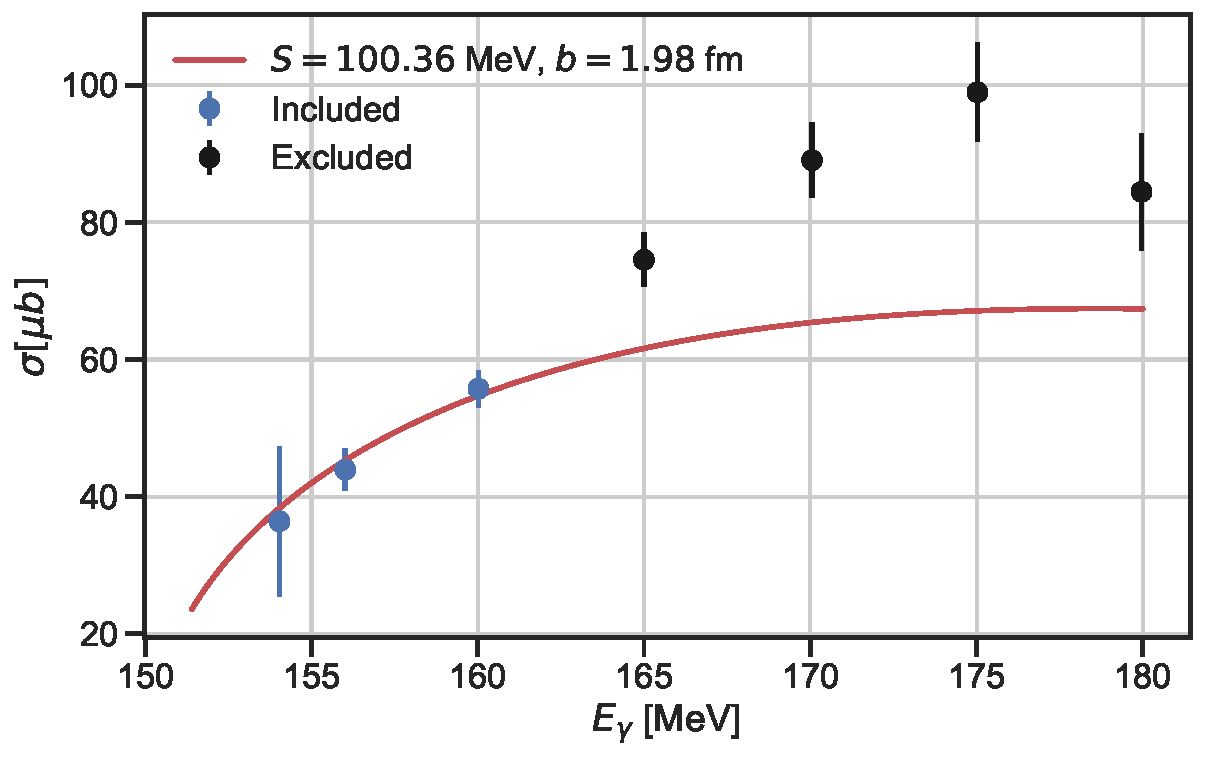
\includegraphics[width=\linewidth]{Figures/dipole_approximation.pdf}
	\end{sidecaption}
\end{figure}
The parameters $S$ and $b$ seem reasonable, but more importantly, we are interested in the relative weight coming from the $N\pi$ component in the wave function and the virtual pions' contribution to the dressed proton. This corresponds to solving the equations in \eqref{system} with the new parameters. The contribution to the wave function is calculated as follows
\begin{align}
	\int_V \text{d}^3R \int_V \text{d}^3 r \, \abs{\psi_{N\pi}}^2 &= 4\pi \int_0^\infty \text{d}r \, \phi(r)^2r^4\\
	&= 0.69
\end{align}
using \eqref{pionnuc} and considering only the $\pi^+$ component in $\vec{\pi}$. The energy is calculated, which yields
\begin{equation}
	E_{\text{virtual pions}} = -449 \, \text{MeV}.
\end{equation}
Note here that we have used two approximations that limit \eqref{dipoletotalcross} to energies very close to the threshold. We need a more general expression for the cross-section and more data points to test the model's validity further. This means we have to consider the exact matrix element for the transition and consider the photoproduction of neutral pions off protons since this is the most experimentally investigated photoproduction process. 
\section{Exact Matrix Element}\label{sec:exact}
In section \ref{sec:dipoleapprox} we looked at how to use the model described in section \ref{sec:model} to get an expression for the cross-section, which was compared to experimental data. More specifically, we used the dipole approximation, which introduces a trade-off between the difficulty of the calculations and the regime in which our solution is valid. We expect the dipole approximation to hold for energies just above the threshold. To both validate and generalize this result, we now make a different approach and calculate the exact cross-section and also consider recoil effects and apply this approach to the four photoproduction processes using the density of states in the non-relativistic and relativistic limit. Strictly speaking, recoil effects should also be considered in section \ref{sec:dipoleapprox} since the mass ratio between the nucleon and the pion cannot be assumed to yield a stationary nucleon after the pion photoproduction process.  
\begin{marginfigure}
	\centering
	

\tikzset{every picture/.style={line width=0.75pt}} %set default line width to 0.75pt        

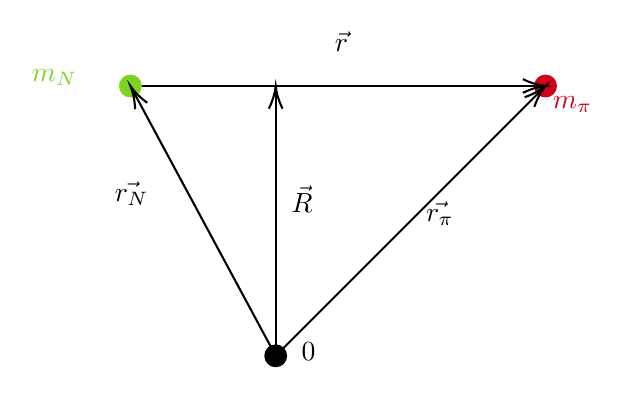
\begin{tikzpicture}[x=0.75pt,y=0.75pt,yscale=-1,xscale=1]
	%uncomment if require: \path (0,300); %set diagram left start at 0, and has height of 300
	
	%Flowchart: Connector [id:dp9827455772611288] 
	\draw  [color={rgb, 255:red, 208; green, 2; blue, 27 }  ,draw opacity=1 ][fill={rgb, 255:red, 208; green, 2; blue, 27 }  ,fill opacity=1 ] (315,90) .. controls (315,87.24) and (317.24,85) .. (320,85) .. controls (322.76,85) and (325,87.24) .. (325,90) .. controls (325,92.76) and (322.76,95) .. (320,95) .. controls (317.24,95) and (315,92.76) .. (315,90) -- cycle ;
	%Straight Lines [id:da5093684133345362] 
	\draw    (125,90) -- (318,90) ;
	\draw [shift={(320,90)}, rotate = 180] [color={rgb, 255:red, 0; green, 0; blue, 0 }  ][line width=0.75]    (10.93,-3.29) .. controls (6.95,-1.4) and (3.31,-0.3) .. (0,0) .. controls (3.31,0.3) and (6.95,1.4) .. (10.93,3.29)   ;
	%Straight Lines [id:da04984112064582158] 
	\draw    (190,220) -- (190,92) ;
	\draw [shift={(190,90)}, rotate = 90] [color={rgb, 255:red, 0; green, 0; blue, 0 }  ][line width=0.75]    (10.93,-3.29) .. controls (6.95,-1.4) and (3.31,-0.3) .. (0,0) .. controls (3.31,0.3) and (6.95,1.4) .. (10.93,3.29)   ;
	%Straight Lines [id:da13661676787341415] 
	\draw    (190,220) -- (318.59,91.41) ;
	\draw [shift={(320,90)}, rotate = 135] [color={rgb, 255:red, 0; green, 0; blue, 0 }  ][line width=0.75]    (10.93,-3.29) .. controls (6.95,-1.4) and (3.31,-0.3) .. (0,0) .. controls (3.31,0.3) and (6.95,1.4) .. (10.93,3.29)   ;
	%Flowchart: Connector [id:dp37210275318157304] 
	\draw  [color={rgb, 255:red, 126; green, 211; blue, 33 }  ,draw opacity=1 ][fill={rgb, 255:red, 126; green, 211; blue, 33 }  ,fill opacity=1 ] (115,90) .. controls (115,87.24) and (117.24,85) .. (120,85) .. controls (122.76,85) and (125,87.24) .. (125,90) .. controls (125,92.76) and (122.76,95) .. (120,95) .. controls (117.24,95) and (115,92.76) .. (115,90) -- cycle ;
	%Straight Lines [id:da8769015497622031] 
	\draw    (190,220) -- (120.95,91.76) ;
	\draw [shift={(120,90)}, rotate = 61.7] [color={rgb, 255:red, 0; green, 0; blue, 0 }  ][line width=0.75]    (10.93,-3.29) .. controls (6.95,-1.4) and (3.31,-0.3) .. (0,0) .. controls (3.31,0.3) and (6.95,1.4) .. (10.93,3.29)   ;
	%Flowchart: Connector [id:dp5562170943538245] 
	\draw  [color={rgb, 255:red, 0; green, 0; blue, 0 }  ,draw opacity=1 ][fill={rgb, 255:red, 0; green, 0; blue, 0 }  ,fill opacity=1 ] (185,220) .. controls (185,217.24) and (187.24,215) .. (190,215) .. controls (192.76,215) and (195,217.24) .. (195,220) .. controls (195,222.76) and (192.76,225) .. (190,225) .. controls (187.24,225) and (185,222.76) .. (185,220) -- cycle ;
	
	% Text Node
	\draw (71,80.4) node [anchor=north west][inner sep=0.75pt]  [color={rgb, 255:red, 126; green, 211; blue, 33 }  ,opacity=1 ]  {$m_{N}$};
	% Text Node
	\draw (322,93.4) node [anchor=north west][inner sep=0.75pt]  [color={rgb, 255:red, 208; green, 2; blue, 27 }  ,opacity=1 ]  {$m_{\pi }$};
	% Text Node
	\draw (196,136.4) node [anchor=north west][inner sep=0.75pt]    {$\vec{R}$};
	% Text Node
	\draw (261,144.4) node [anchor=north west][inner sep=0.75pt]    {$\vec{r_{\pi }}$};
	% Text Node
	\draw (111,134.4) node [anchor=north west][inner sep=0.75pt]    {$\vec{r_{N}}$};
	% Text Node
	\draw (217,62.4) node [anchor=north west][inner sep=0.75pt]    {$\vec{r}$};
	% Text Node
	\draw (201,212.4) node [anchor=north west][inner sep=0.75pt]    {$0$};
	
	
\end{tikzpicture}
	\caption{Sketch of the system. Here $\vec{r}_N$ is the coordinate of the proton and $\vec{r}_\pi$ is the coordinate of the pion. The relative coordinate is given by $\vec{r}=\vec{r}_\pi-\vec{r}_p$ and the coordinate of the center-of-mass is $\vec{R}=(m_p \vec{r}_p+m_\pi\vec{r}_\pi)/(m_p+m_\pi)$. The total mass is denoted $M_{p\pi}=m_p+m_\pi$.}
	\label{JacobiIllustration}
\end{marginfigure}
To calculate the exact matrix elements we consider a non-relativistic system of particles interacting with the electromagnetic field as described in section \ref{RadMatter}. We have to keep in mind that equation \eqref{RadiationHamil} describes how a particle with charge interacts with the electromagnetic field. This means if we consider a process where the initial state is a dressed neutron, the pion must be responsible for the interaction with the electromagnetic field. We will consider the four pion photoproduction processes separately even though the calculations are very similar. In general, we will consider a system illustrated in figure \ref{JacobiIllustration}, which shows the pion-nucleon system, and in terms of the Jacobi coordinates, we get the following expressions for the coordinates of the particles
\begin{align} \label{Coordinates}
	\vec{r}_N = \vec{R}-\frac{m_\pi}{M_{N\pi}}\vec{r} \\
	\vec{r}_\pi = \vec{R}+\frac{m_N}{M_{N\pi}}\vec{r},
\end{align}
where $\vec{R}$ is the coordinate of the center of mass of the pion-nucleon system given by
\begin{equation} \label{Rvec}
	\vec{R}=\frac{m_N \vec{r}_N+m_\pi \vec{r}_\pi}{M_{N\pi}}, \quad M_{N\pi} = m_N+m_\pi.
\end{equation}
The relative coordinate is given by
\begin{equation} \label{rvec}
	\vec{r} = \vec{r}_\pi-\vec{r}_N.
\end{equation}
The general approach is the same as in section \ref{sec:DressingofProton} where we want to use Fermi's golden rule to calculate the total cross-section. In this section, we also consider the impact of changing the density of states to the relativistic case. Furthermore, we estimate the relative weight of the pion component in the wave function of the dressed nucleon. We do this by introducing the following
\begin{equation} \label{relativeweight}
	C(\psi_{N\pi}) = \int_V \text{d}^3 R \int_V \text{d}^3 r \, \abs{\psi_{N\pi}}^2,
\end{equation}
where per construction of the model, this is dimensionless. We also introduce a parameter to estimate the virtual pions' contribution to the mass of the dressed nucleon. This will be denoted $\Pi$ and corresponds to the energy found by solving \eqref{system}.

\subsection{Neutral Pion Phototoproduction off Protons}\label{sec:NeutralOffProton}
We are considering the process 
\begin{equation} \label{prod1}
	p\gamma \rightarrow \pi^0 p,
\end{equation}
where the proton interacts with the electromagnetic field. From equation \eqref{RadiationHamil} we get
\begin{equation} \label{1trans}
	H^{(1)} = -\frac{e}{m_pc} \vec{A}(\vec{r}_p,t)\cdot \vec{p}_p,
\end{equation}
where $\vec{p}_p$ is the momentum operator of the proton.  Equation \eqref{1trans} can be rewritten in terms of the relative coordinates
\begin{equation} \label{1rela}
	H^{(1)} = -\frac{e}{m_p c}\vec{A}\left( \vec{R}-\frac{m_\pi}{M_{p\pi}}\vec{r,t}\right) \cdot \left( \frac{m_p}{M_{p\pi}}\vec{P}-\vec{p}\right)
\end{equation}
In equation \eqref{prod1}, the initial state consists of a dressed proton and a plane wave photon in the state $a_{\vec{k},\lambda}^\dagger\ket{0}$ where $\vec{k}$ is the wave number and $\lambda$ the polarisation index. The final state consists of a proton and a $\pi^0$ in a relative plane wave motion. The electromagnetic part of the matrix element is
\begin{align} \label{eletrans}
	-\frac{e}{m_p c}\mel{0}{\vec{A}(\vec{r}_p,t)a^\dagger_{\vec{k},\lambda}}{0} &= -\frac{e}{m_p c}\sqrt{\frac{2\pi\hbar}{\omega_k V}}\vec{e}_{\vec{k},\lambda} \text{e}^{i\vec{k}\cdot \vec{r}_p-i\omega_k t} \\
	&=  -\frac{e}{m_p c}\sqrt{\frac{2\pi\hbar}{\omega_k V}}\vec{e}_{\vec{k},\lambda} \text{e}^{i\vec{k}( \vec{R}-\frac{m_\pi}{M_{p\pi}}\vec{r})-i\omega_k t}.
\end{align}
We now return to equation \ref{1rela} where we set $\vec{P}=0$, which corresponds to moving to the lab frame, and the matrix element needed for Fermi's golden rule is given by
\begin{equation}\label{MatrixSpinupdown} 
	\mathcal{M}^{(\uparrow\downarrow)} = \frac{e}{m_p} \sqrt{\frac{2\pi\hbar}{\omega_{\vec{k}}V}} \mel*{(\uparrow\downarrow)p\pi^0 \frac{\text{e}^{i\vec{q}\cdot \vec{r}}}{\sqrt{V}}\frac{\text{e}^{i\vec{Q}\cdot \vec{r}}}{\sqrt{V}}}{\text{e}^{i\vec{k}(\vec{R}-\frac{m_\pi}{M_{p\pi}}\vec{r})}(\vec{e}_{\vec{k},\lambda}\vec{p})}{\psi_{N\pi}} ,
\end{equation}
where $\vec{q}$ is the wave number of the relative pion-proton system and $\vec{Q}=\vec{k}$ is the recoil. Looking at the isospin coefficient from equation \eqref{isocoeff}, which is the factor that separates neutral pions from charged pions aside from the mass difference\footnote{$\mel{p\pi^0}{\vec{\tau}\cdot\vec{\pi}}{p}=1$}. Inserting \eqref{pionnuc} and using that volume condition yields the following expression\footnote{$\int \text{d}^3R \, \text{e}^{i\vec{k}\cdot\vec{R}}=V$}
\begin{equation} \label{MatrixSpinupdown2}
	\mathcal{M}^{(\uparrow\downarrow)} = \frac{e}{m_p} \sqrt{\frac{2\pi\hbar}{\omega_{\vec{k}}V}} \mel*{(\uparrow\downarrow)p\pi^0 \frac{\text{e}^{i\vec{q}\cdot \vec{r}}}{\sqrt{V}}}{\text{e}^{-i\frac{m_\pi}{M_{p\pi}}\vec{k}\cdot\vec{r}}(\vec{e}_{\vec{k},\lambda}\vec{p})}{(\vec{\tau}\cdot\vec{\pi})(\vec{\sigma}\cdot\vec{r})\phi(r) \frac{p\uparrow}{\sqrt{V}}} 
\end{equation}
Defining a new vector, $\vec{s}=\vec{q}+\frac{m_\pi}{M_{p\pi}}\vec{k}$ yields
\begin{equation}\label{doublematrix}
	\mathcal{M}^{(\uparrow\downarrow)} = \frac{-e}{m_\pi} \sqrt{\frac{2\pi\hbar}{\omega_{\vec{k}}}} \frac{1}{V} \mel{(\uparrow \downarrow)}{\mel*{\text{e}^{i\vec{s}\cdot\vec{r}}}{(\vec{e}_{\vec{k},\lambda}\vec{p})(\vec{\sigma}\cdot\vec{r})}{\phi(r)}}{\uparrow}
\end{equation}
Note the different inner products. We now consider the innermost matrix element in equation \eqref{doublematrix} where the momentum operator is inserted
\begin{align}
	\mel*{\text{e}^{i\vec{s}\cdot\vec{r}}}{(\vec{e}_{\vec{k},\lambda}\frac{\partial}{\partial \vec{r}})\sigmar}{\phi(r)} &=+i(\vec{e}_{\vec{k},\lambda}\cdot \vec{s}) \int \text{d}^3 r \, \text{e}^{i\vec{s}\cdot\vec{r}}\sigmar \phi(r) \\ 
	&= -i(\vec{e}_{\vec{k},\lambda}\cdot \vec{s}) \int \text{d}^3 r \, 3 i j_1(sr) \frac{\vec{s}\cdot \vec{r}}{sr}\sigmar \phi(r)  \label{planebob}\\
	&= (\vec{e}_{\vec{k},\lambda}\cdot \vec{s})\sigmar \underbrace{\frac{4\pi}{s} \int_0^\infty \text{d}r \, r^3 j_1(sr) \phi(r)}_{F(s)} \label{unitbob} \\
	&= (\vec{e}_{\vec{k},\lambda}\cdot \vec{s})\sigmar F(s).
\end{align}
Where we used the spherical Bessel decomposition \eqref{sphericalbesseldecomp} in equation \eqref{planebob}. In equation \eqref{unitbob} we considered the angular averaging of two coordinates variables\footnote{$\int \text{d}\Omega \, n_k n_l =\frac{4\pi}{3}\delta_{kl}$, which means $\int \text{d}\Omega \, r_k r_l =\frac{4\pi r^2}{3}\delta_{kl}$, where $n$ is a unit vector.}.
We now have an expression for the innermost matrix element in equation \eqref{doublematrix}, which depends on the wave function $\phi(r)$. This is where the two parameters $S$ and $b$ enter, and ultimately these are the parameters we want to extract. Returning to the matrix element \eqref{doublematrix}
\begin{align}
	\mathcal{M^{(\uparrow\downarrow)}} &= \frac{ie\hbar}{m_p}\sqrt{\frac{2\pi \hbar}{\omega_k}}\frac{1}{V}\mel*{(\uparrow\downarrow)}{(\vec{e}_{\vec{k},\lambda}\cdot\vec{s})F(s)}{\uparrow} \\
	&=\frac{ie\hbar}{m_p}\sqrt{\frac{2\pi \hbar}{\omega_k}}\frac{1}{V} (\vec{e}_{\vec{k},\lambda}\cdot\vec{s})\mel*{(\uparrow\downarrow)}{\sigmar}{\uparrow}F(s),
\end{align}
which leads to the following expression for the norm square of equation \eqref{doublematrix}. We do this step already to use a completeness relation for the polarization.
\begin{equation} \label{matrixspinupdownabs}
	\abs{\mathcal{M}^{(\uparrow\downarrow)}}^2 = \frac{2\pi\hbar^3e^2}{m_p^2\omega_k V^2} \abs{\evec\cdot \vec{s}}^2 \abs{\mel*{(\uparrow\downarrow)}{(\vec{\sigma}\cdot \vec{s})}{\uparrow}}^2 F(s)^2,
\end{equation}
and now calculating
\begin{align} \label{sumoverpol}
	\sum_\lambda \abs{(\evec \cdot \vec{s})}^2 &= \sum_\lambda (\evec^*\cdot \vec{s})(\evec\cdot\vec{s}) \\
	&= s^2 -\frac{(\vec{k}\cdot \vec{s})^2}{k^2} \\
	&= q^2 -\frac{(\vec{k}\cdot \vec{q})^2}{k^2} \\
	&= q^2 \sin^2(\theta_q),\label{finalsum}
\end{align}
where $\theta_q$ is the angle between $\vec{k}$ and $\vec{q}$, and we now have an angular dependency originating from the dot product. This step also assumes the target is unpolarised since we sum over the spin states of the proton. The subscript $q$ is used to emphasize that this is relative to the final state momentum, also mentioned in section \ref{sec:densityofstates}. The final missing term is calculated by summing over the final proton spin states using \eqref{spinmatrix}
\begin{equation} \label{spinsum}
	\sum_{(\uparrow\downarrow)} \abs{\mel*{(\uparrow\downarrow)}{(\vec{\sigma}\cdot\vec{s})}{\uparrow}}^2 = s^2
\end{equation}
Using the final two expressions equation \eqref{finalsum} and \eqref{spinsum} with equation \eqref{matrixspinupdownabs} and remembering the factor $1/2$ from the spin states
\begin{equation} \label{absmatrixexact}
	\frac{1}{2}\sum_{\lambda,(\uparrow\downarrow)} \abs{\mathcal{M}_{fi}}^2 = \frac{\pi e^2\hbar^3}{V^2 m_p^2}\frac{1}{\omega_k} q^2\sin^2(\theta) s^2 F(s)^2.
\end{equation}
According to Fermi's golden rule, the transition probability is given by
\begin{align}\label{Fermisgolden}
	\text{d}\omega &= \frac{2\pi}{\hbar}\abs{\mathcal{M}}^2\text{d}\rho,
\end{align}
where we can use both expressions for the density of states. We can either use the relativistic equation \eqref{derivative} or the non-relativistic equation \eqref{nonreladensity}. We will use the relativistic expression as an example but show both results at the end of the section. This leads to the final transition probability
\begin{align}
	\text{d}\omega^0 = \frac{e^2c}{8\pi V}\frac{}{m_p^2 c^4}\frac{\text{d}(\hbar c q)^2}{\text{d}E_q}\frac{q^3}{k} \sin^2(\theta_q) s^2 F(s)^2 \text{d}\Omega_q
\end{align}
which leads to the following expression for the differential cross section by considering the time it takes the photon to cross the volume, $V$.
\begin{align}\label{exactdiffcross}
	\frac{\text{d}\sigma^0(E_q,\theta_q)}{\text{d}\Omega_q} &= \frac{e^2}{8\pi}\frac{1}{m_p^2c^4}\frac{q^3}{k}\frac{\text{d}(\hbar c q)^2}{\text{d}E_q}\sin^2(\theta_q) s^2 F(s)^2,
\end{align}
where the superscript is used to indicate photoproduction of neutral pions. To get the total cross-section, we integrate all angles
\begin{align} \label{exactcross}
	\sigma^0 & = 2\pi \int_0^\pi \text{d}\theta_q \, \sin(\theta_q) \frac{\text{d}\sigma^0}{\text{d}\Omega_q} \\ &= 2\pi \int_0^\pi \text{d}\theta_q \, \frac{e^2}{8\pi}\frac{1}{m_p^2c^4}\frac{q^3}{k}\frac{\text{d}(\hbar c q)^2}{\text{d}E_q}\sin^3(\theta_q) s^2 F(s)^2 \label{finalcrosser}.
\end{align}
Equation \eqref{finalcrosser} might seem easy to calculate at first, but we have to remember $F(s)$ also contains an angular dependency originating from the magnitude of $\vec{s}$. We now perform a fit of equation \eqref{finalcrosser} to experimental data for the parameters $S$ and $b$. This is shown in figure \ref{fig:crossfitrel} for the relativistic density of states. Data is from  \cite{Schmidt_2001}.
\begin{figure}[H]
	\begin{sidecaption}{Fitted parameters to experimental data for the process $\gamma p \rightarrow \pi^0 p$. The fit parameters for $S,b$ are shown inside the figure. Data is from \cite{Schmidt_2001}}[fig:crossfitrel]
		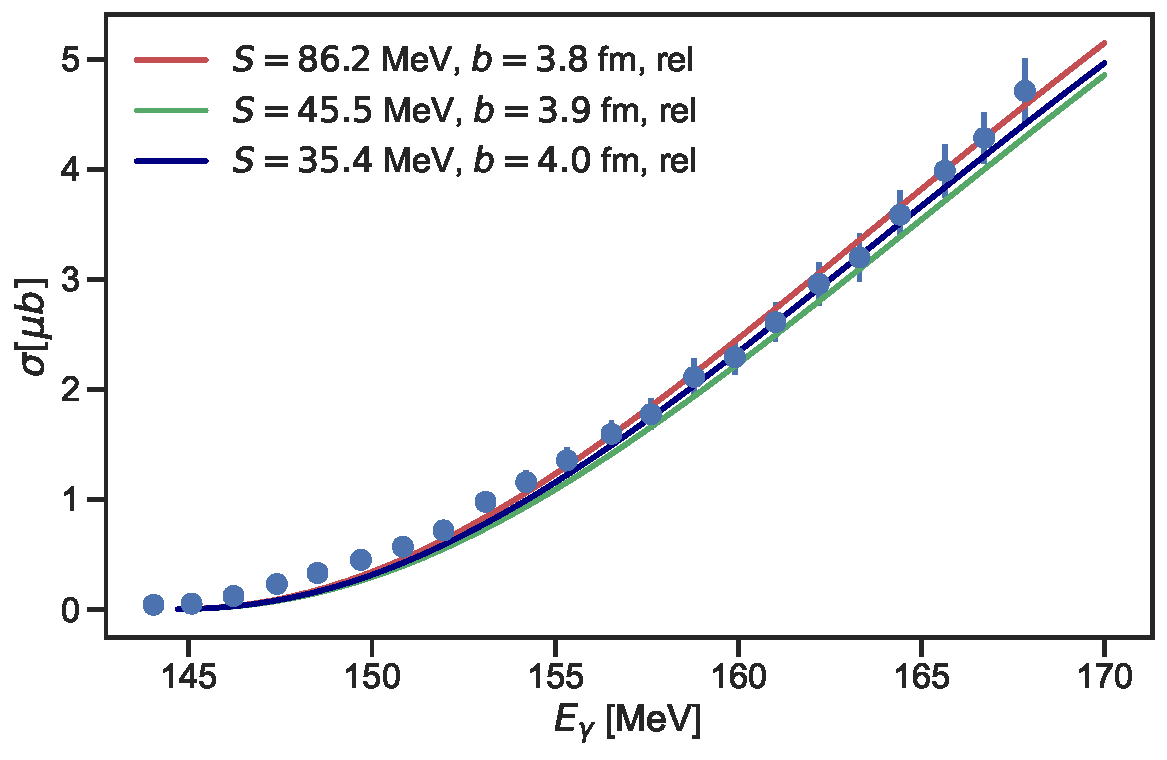
\includegraphics[width=\linewidth]{Figures/crossfit_rel.pdf}
	\end{sidecaption}
\end{figure}
We see that the model with explicit pions can reproduce experimental data for at least three sets of parameters. The same figure can be reproduced for the non-relativistic density of states \eqref{nonreladensity} where the total cross section is given by
\begin{equation} \label{nonrelcrossfit}
	\sigma^0 = 2\pi \int_0^\pi \text{d}\theta_q \, \frac{e^2}{4\pi}\frac{\mu_{p\pi}c^2}{m_p^2 c^4}\frac{q^3}{k}\sin^3(\theta_q)s^2 F(s)^2.
\end{equation} 
This is shown in figure \ref{fig:crossfitnonrel}
\begin{figure}[H]
	\begin{sidecaption}{Fitted parameters to experimental data for the process $\gamma p \rightarrow \pi^0 p$. The fit parameters for $S,b$ are shown inside the figure.}[fig:crossfitnonrel]
		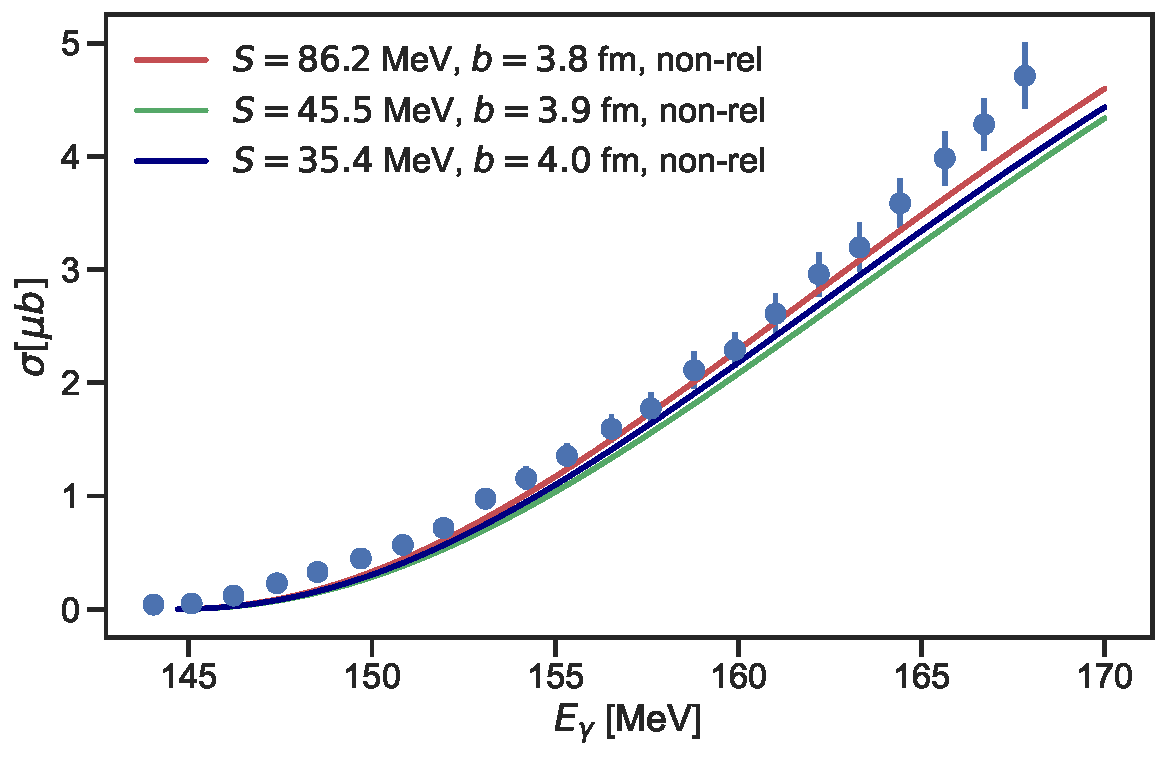
\includegraphics[width=\linewidth]{Figures/crossfit_nonrel.pdf} 
	\end{sidecaption}
\end{figure}
The total cross-section falls off too quickly as relativistic effects become more important. In equation \eqref{exactdiffcross}, we have an expression for the angular dependency. This means that for some photon energy, we get an angular distribution. Figure \ref{fig:angular151} shows the differential cross section as a function of the angle $\theta_q$ compared to experimental data. Data is from \cite{BeckPion}  
\begin{figure}[H]
	\begin{sidecaption}{Note the dependency is not $\sin(\theta_q)^2$ since there is a contribution from $F(s)$ as well.}[fig:angular151]
		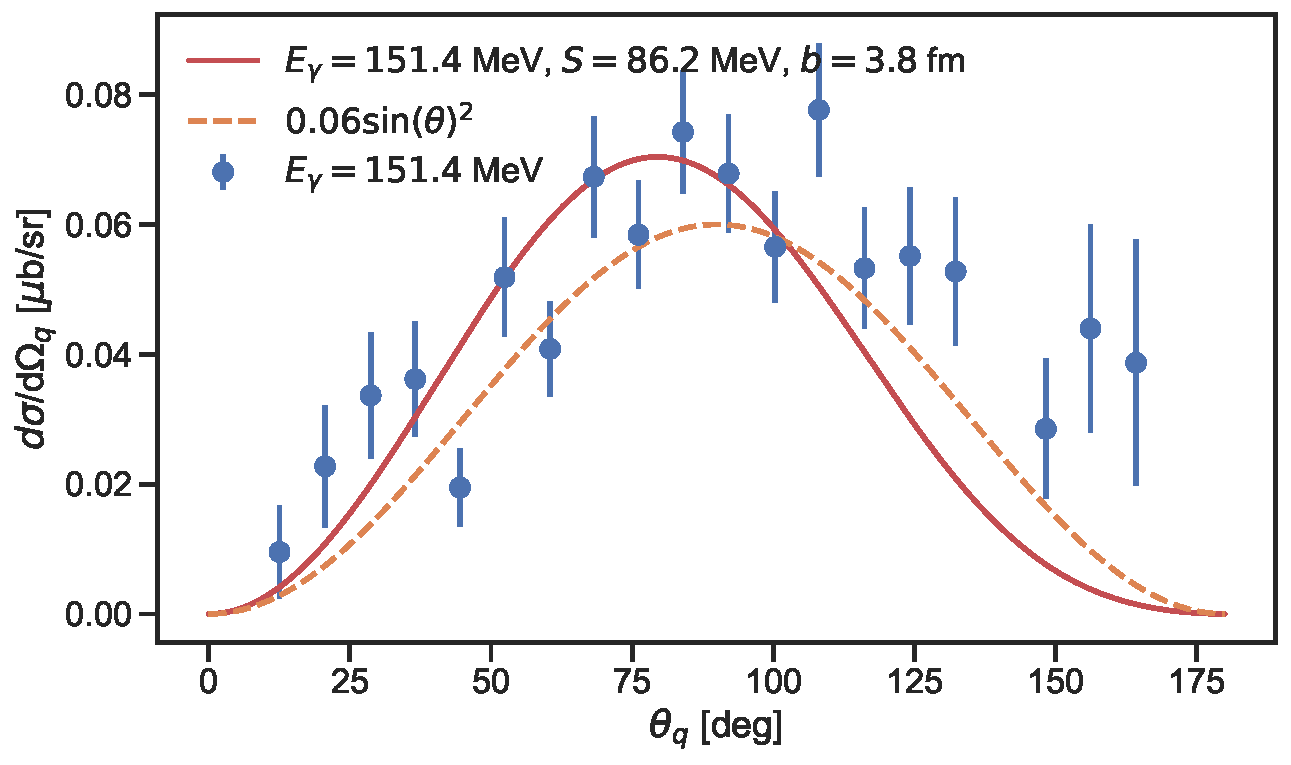
\includegraphics[width=\linewidth]{Figures/DiffCross151_rel.pdf}
	\end{sidecaption}
\end{figure}
Figure \ref{fig:angular151} also shows how the angular dependency is not a $\sin(\theta_q)^2$ but also has some contribution from $F(s)$. Figure \ref{fig:MultipleEnergies} shows multiple different photon energies.
\begin{figure}[H]
	\begin{sidecaption}{Multiple energies}[fig:MultipleEnergies]
		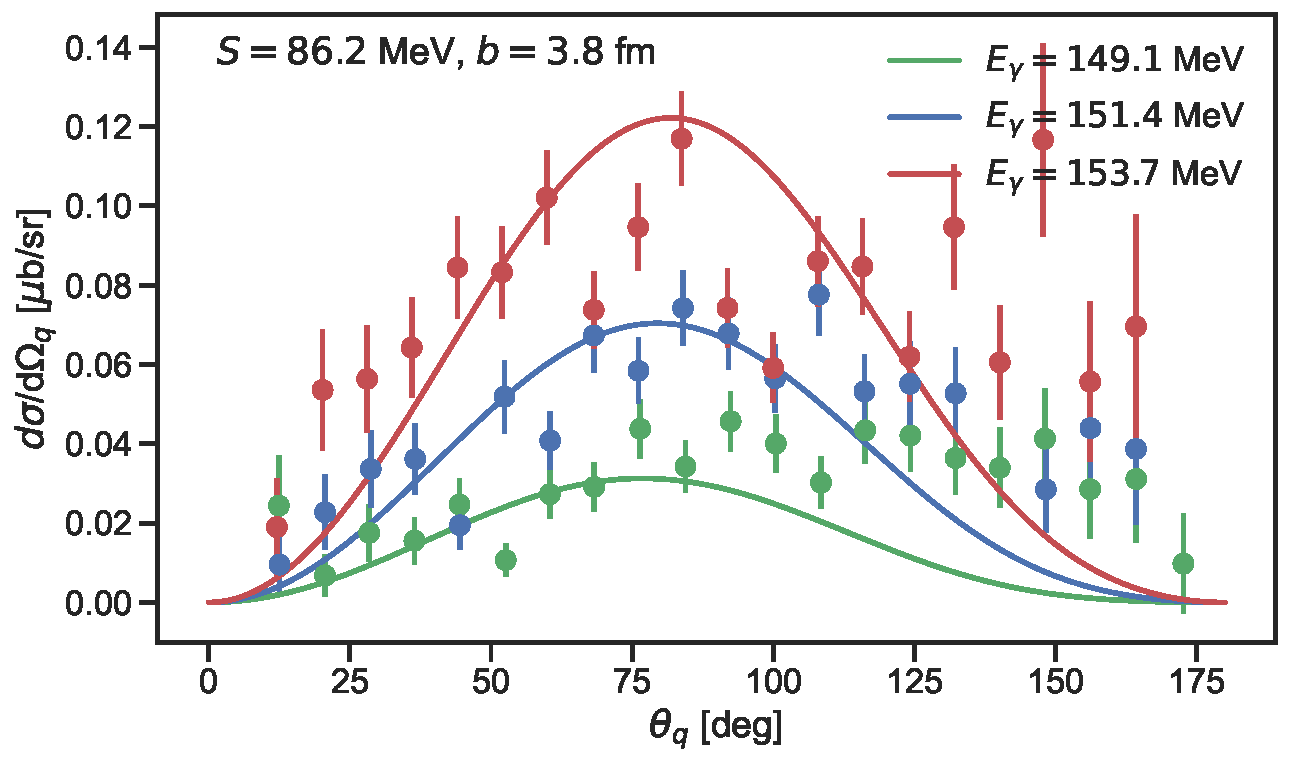
\includegraphics[width=\linewidth]{Figures/MultiDiffcross_rel.pdf}
	\end{sidecaption}
\end{figure}
Figures for the differential cross-section using different parameters and using the non-relativistic density of states are shown in appendix \ref{sec:Angular}.

The final thing we need to consider is the relative weight of the $\pi^0$ component in the wave function of the dressed proton. As in section \ref{sec:dipoleapprox} it is calculated as 
\begin{align}
	C(\psi_{N\pi^0})= \int_V \text{d}^3R \int_V \text{d}^3 r \, \abs{\psi_{N\pi}}^2 &= 4\pi \int_0^\infty \text{d}r \, \phi(r)^2r^4 \\
	&= 0.258, 
\end{align}
for the green line. The virtual pions contribute $649.4$ MeV

For the three sets of parameters shown in figure \ref{fig:crossfitrel}, the contribution to the wave function from the $\pi^0$ is

\begin{figure}[H]
	\begin{sidecaption}{Fitted parameters to experimental data for the process $\gamma p \rightarrow \pi^0 p$. The fit parameters for $S,b$ are shown inside the figure.}[fig:ContributionPlot]
		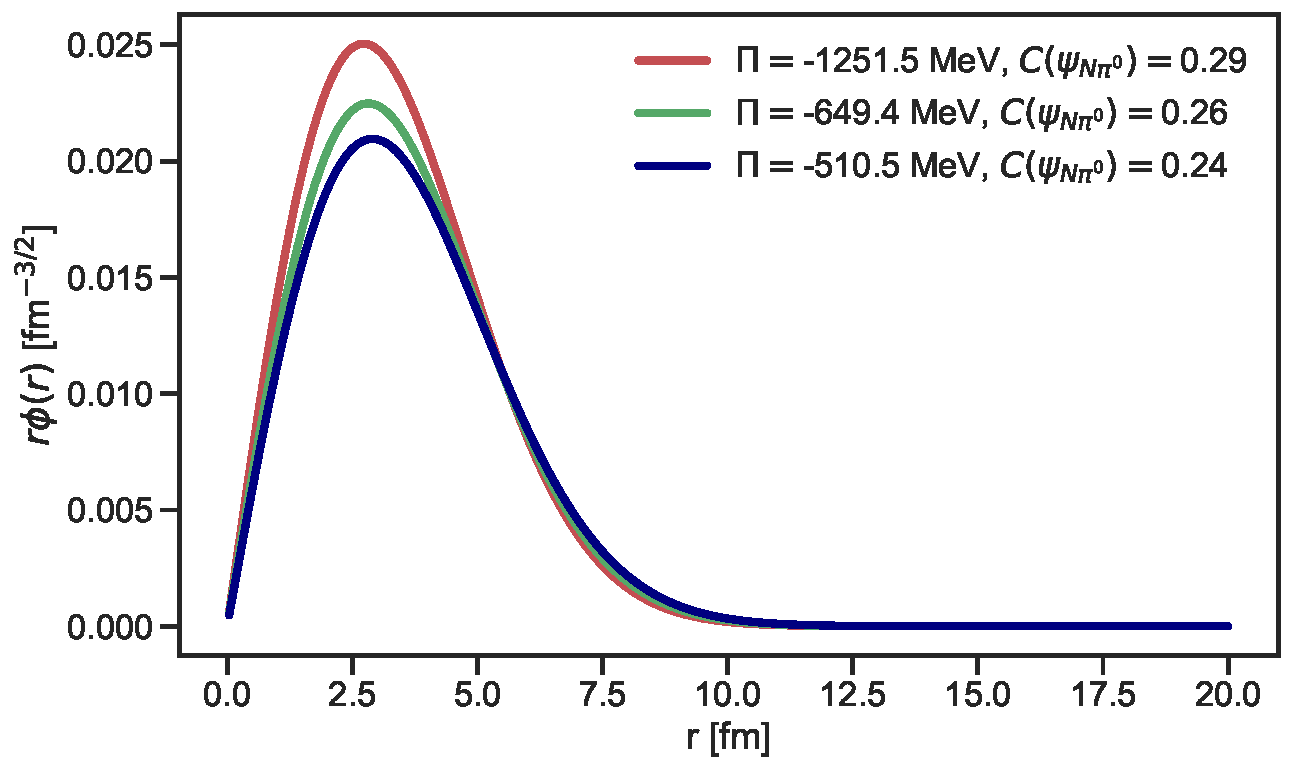
\includegraphics[width=\linewidth]{Figures/ContributionPlot.pdf} 
	\end{sidecaption}
\end{figure}
\subsection{Neutral Pion Phototoproduction off Neutrons}
We now consider the process 
\begin{equation} \label{process2}
	n\gamma \rightarrow \pi^0 n,
\end{equation}
which is very similar to the process in section \ref{sec:NeutralOffProton}. The key difference is that now the pion is responsible for the interaction with the electromagnetic field, and hence equation \eqref{RadiationHamil} depends on the pion 
\begin{equation} \label{RadiNeutron}
	H^{(1)} = -\frac{e}{m_\pi c}\vec{A}(\vec{r}_\pi,t)\cdot\vec{p}_\pi	
\end{equation}
This changes two things in comparison to equation \eqref{exactdiffcross}. The mass of the proton becomes the mass of the pion, and the wave number vector becomes $\vec{s}=\vec{q}-\frac{m_n}{M_{n\pi}}\vec{k}$, where $n$ is the mass of the neutron. Therefore the final expression for the total cross-section becomes 
\begin{equation} \label{totalcrossneutron}
	\frac{\text{d}\sigma^0(E_q,\theta_q)}{\text{d}\Omega_q} = \frac{e^2}{8\pi}\frac{1}{m_\pi^2c^4}\frac{q^3}{k}\frac{\text{d}(\hbar c q)^2}{\text{d}E_q}\sin^2(\theta_q) s^2 F(s)^2.
\end{equation}
Unfortunately, no experimental data exists such that a fit can be performed. A comparison with other theoretical models is made to test the validity of equation \ref{totalcrossneutron}. Specifically, we test if the expression can replicate other theoretical predictions for a given set of $S$ and $b$. The other models are \cite{MAINZA2} and \cite{MAID2017}.
\begin{figure}[H]
    \begin{sidecaption}{The process $\gamma n \rightarrow \pi^0 n$ with the same parameters as for neutral pion photoproduction off protons.}[fig:neutralpionsoffneutrons]
    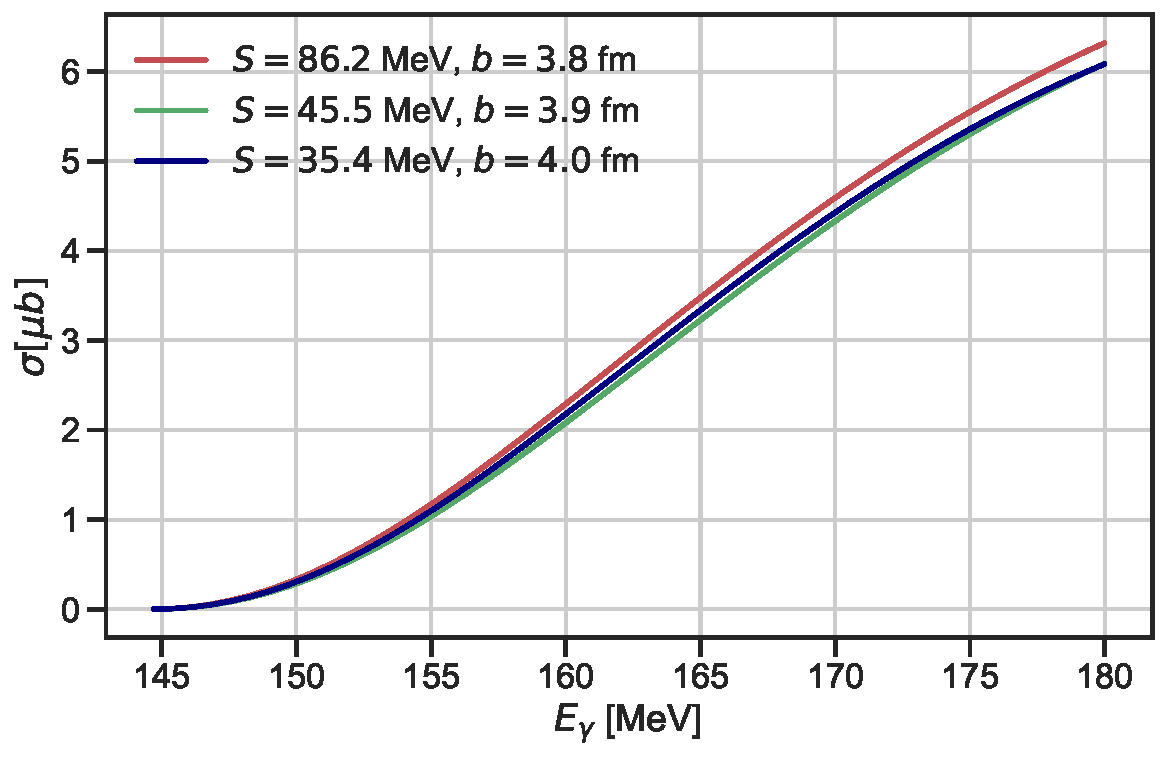
\includegraphics[width=\linewidth]{Figures/NeutralPionsOffNeutrons.pdf}
    \end{sidecaption}
\end{figure}
\subsection{Charged Pion Phototoproduction off Protons}
We now consider the process involving charged pions. Specifically,
\begin{equation} \label{charged1}
	p\gamma \rightarrow \pi^+ n,
\end{equation}
which is very similar to equation \eqref{prod1} except we have to consider the isospin coefficient. We do this by considering equation \eqref{isocoeff} which brings a factor 2 to the differential cross-section. This means the total cross-section is given by
\begin{equation} \label{totcross3}
	\sigma^+ =  2\pi \int_0^\pi \text{d}\theta_q \, \frac{e^2}{4\pi}\frac{1}{m_p^2c^4}\frac{q^3}{k}\frac{\text{d}(\hbar c q)^2}{\text{d}E_q}\sin^3(\theta_q) s^2 F(s)^2,
\end{equation}
where the $+$ indicates the production of positively charged pions. We once again fit equation \eqref{totcross3} to experimental data. The result can be seen on figure \ref{fig:ChargedPionOffProton} where the data is from 
\begin{figure}[H]
	\begin{sidecaption}{Data from \cite{PionOffNeutron2}}[fig:ChargedPionOffProton]
		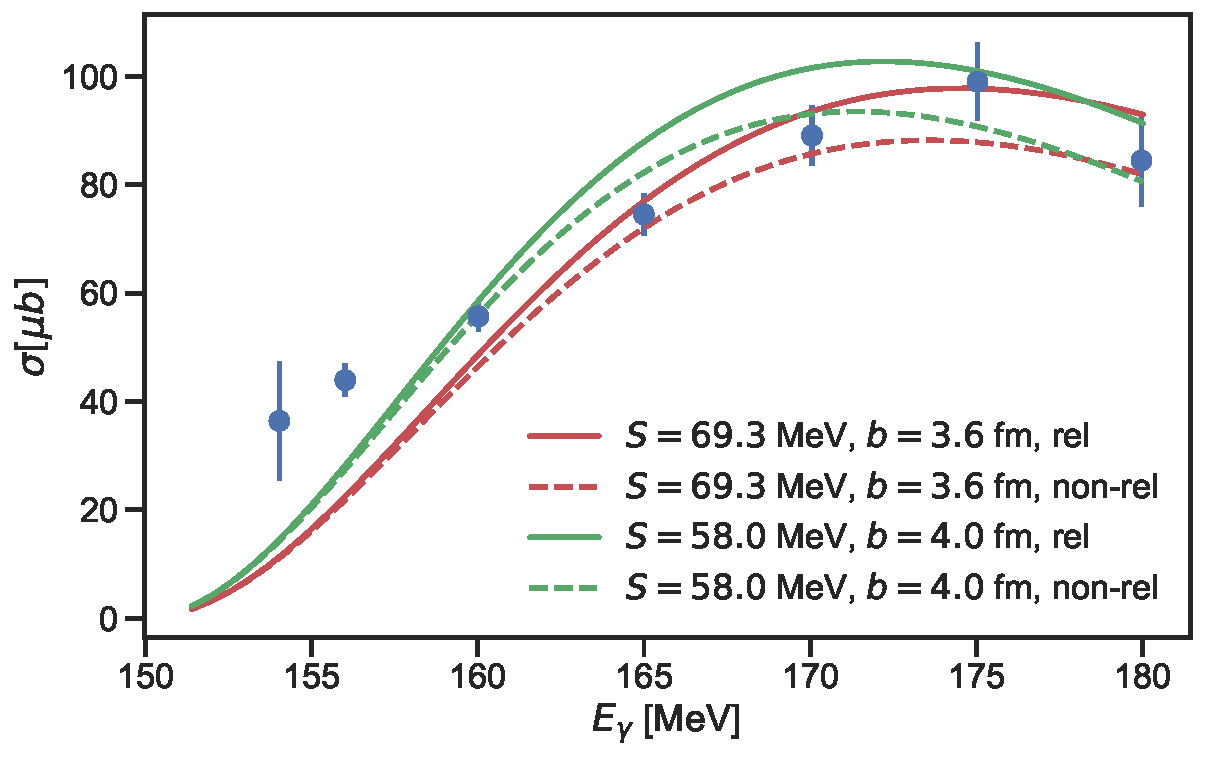
\includegraphics[width=\linewidth]{Figures/ChargedPionOffProtonExact.pdf}
	\end{sidecaption}
\end{figure}
Figure \ref{fig:ChargedPionOffProton} shows the model has some difficu
\begin{figure}[H]
	\begin{sidecaption}{Contributions}[fig:ContributionPlotPlus]
		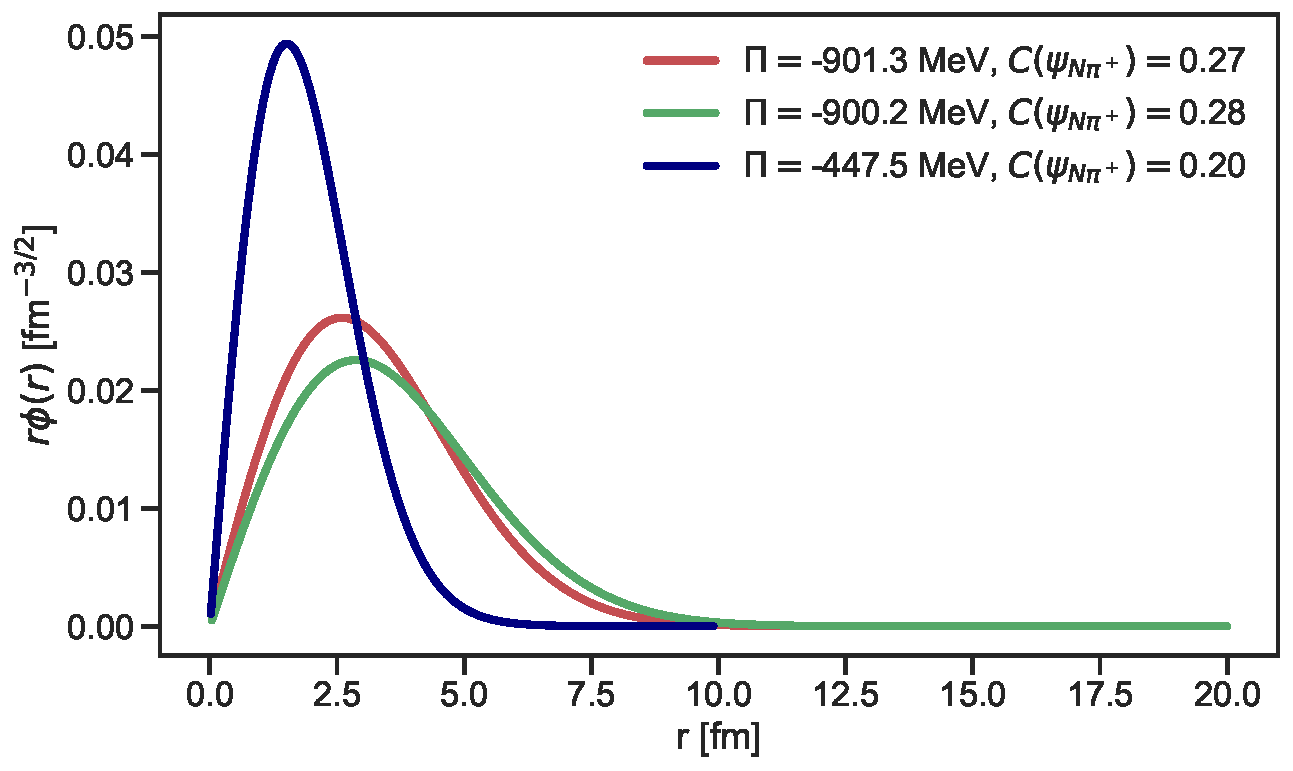
\includegraphics[width=\linewidth]{Figures/ContributionPlotPiPlus.pdf}
	\end{sidecaption}
\end{figure}}
\subsection{Charged Pion Phototoproduction off Neutrons}
\begin{figure}[H]
	\begin{sidecaption}{d.}[fig:ChargedPionOffNeutron]
		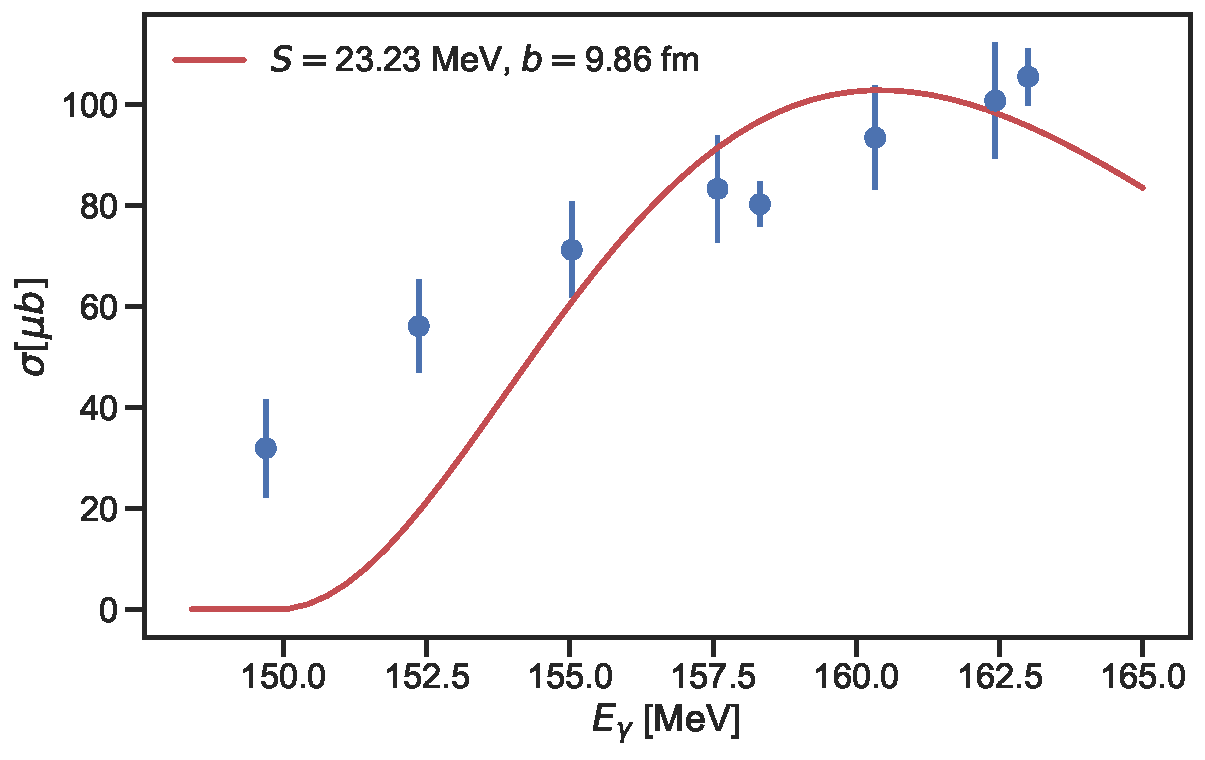
\includegraphics[width=\linewidth]{Figures/ChargedPionOffNeutron.pdf}
	\end{sidecaption}
\end{figure}